\documentclass{article}

\usepackage{amsmath}
\usepackage{parskip}
\usepackage{tikz}
\renewcommand{\emph}{\textbf}

\begin{document}

\section{Frame 12 -- Functions of Complex Variables}
\textbf{1(a)} 
The function
\[
	f(z) = \frac{1}{z^2 + 1}
\]
is defined everywhere except where $z^2 + 1 = 0$; ie:
\[
	z \neq \pm i
\]

\textbf{1(b)}
The function
\[
	f(z) = \text{Arg}\Big(\frac{1}{z}\Big)
\]
is defined wherever $\frac{1}{z}$ is defined:
\[
	z \neq 0
\]

\textbf{1(c)}
The function
\[
	f(z) = \frac{z}{z + \bar z}
\]
can be written as
\[
	f(x, y) = \frac{x + iy}{(x + iy) + (x - iy)} = \frac{x + iy}{2x} = \frac{1}{2} + i \frac{y}{x}
\]
so the domain is
\[
	\text{Re}(z) \neq 0
\]

\textbf{1(d)}
The function
\[
	f(z) = \frac{1}{1 - |z|^2}
\]
is equivalent to
\[
	f(r, \theta) = \frac{1}{1 - r^2}
\]
so the domain is
\[
	r \neq 1
\]


\textbf{2}
Substituting $z = x + iy$ gives
\begin{align*}
	f(x, y) &= (x + iy)^3 + (x + iy) + 1 \\
	&= x^3 + 3x^2(iy) + 3x(iy)^2 + (iy)^3 + x + iy + 1 \\
	&= (x^3 - 3xy^2 + x + 1) + i(3x^2y - y^3 + y) 
\intertext{so}
	u(x, y) &= x^3 - 3xy^2 + x + 1 \\
	v(x, y) &= 3x^2y - y^3 + y
\end{align*}


\textbf{3}
Using the two expressions
\begin{align*}
	x &= \frac{z + \bar{z}}{2} \\
	y &= \frac{z - \bar{z}}{2i}
\end{align*}
gives
\begin{align*}
	f(z) &= 
	\Big(\frac{z + \bar{z}}{2}\Big)^2 
	- \Big(\frac{z - \bar{z}}{2i}\Big)^2 
	- 2 \frac{z - \bar{z}}{2i} \\
	& \quad + i\Big[2 \frac{z + \bar{z}}{2} \Big(1 - \frac{z - \bar{z}}{2i}\Big) \Big] \\
% 	
	&= \frac{1}{4} (z^2 + 2z\bar{z} + \bar{z}^2 + z^2 - 2z\bar{z} + \bar{z}^2) 
	+ i z - i \bar{z} \\
	& \quad + i \Big[ z + \bar{z} + \frac{iz^2}{2} - \frac{i\bar{z}^2}{2}\Big] \\
%
	&= \frac{1}{2} (z^2 + \bar{z}^2) + 2iz - \frac{iz^2}{2} + \frac{\bar{z}^2}{2} \\
%
	&= \bar{z}^2 + 2iz
\end{align*}


\textbf{4}
Using
\[
	z = re^{i\theta}
\]
the function can be written as
\begin{align*}
	f(z) &= re^{i\theta} + \frac{1}{re^{i\theta}} \\
	&= re^{i\theta} + \frac{1}{r} e^{-i\theta} \\
	&= (r + \frac{1}{r}) \cos \theta + i(r - \frac{1}{r}) \sin \theta
\end{align*}


\clearpage
\section{Frame 14 -- Mappings by the Exponential Function}
\textbf{1}
We saw earlier that the hyperbolas
\[
	x^2 - y^2 = c_1
\]
map onto the horizontal lines $u = c_1$ and the hyperbolas
\[
	2xy = c_2
\]
map onto the vertical lines $v = c_2$. Thus, a domain on the z-plane that maps onto $1 \le u \le 2$ and $1 \le v \le 2$ is
\[
	1 \le x^2 - y^2 \le 2	\quad	1 \le 2xy \le 2
\]
A sketch of this region is:
\begin{center}
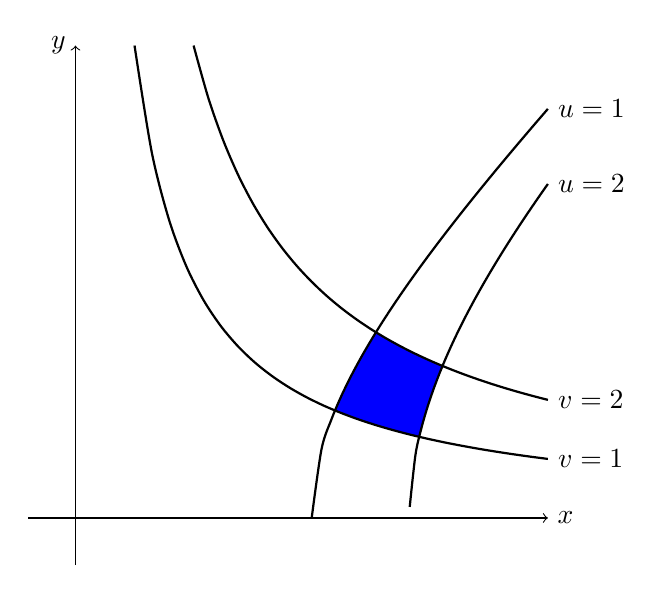
\begin{tikzpicture}[scale=3]
	\draw [->] (-0.2,0) to (2,0) node[right]{$x$};
	\draw [->] (0,-0.2) to (0,2) node[left] {$y$};
	
	\fill [fill=blue]
		plot [domain=1.272:1.554] (\x, {2 / (2*\x)}) --
		plot [domain=1.554:1.455] (\x, {sqrt(\x*\x - 2)}) --
		plot [domain=1.455:1.099] (\x, {1 / (2*\x)}) --
		plot [domain=1.099:1.272] (\x, {sqrt(\x*\x - 1)});
	\draw [thick, domain=0.25:2]  plot [smooth] (\x, {1 / (2*\x)}) node[right]{$v = 1$};
	\draw [thick, domain= 0.5:2]  plot [smooth] (\x, {2 / (2*\x)}) node[right]{$v = 2$};
	\draw [thick, domain=1:2]     plot [smooth] (\x, {sqrt(\x*\x - 1}) node[right]{$u = 1$};
	\draw [thick, domain=1.415:2] plot [smooth] (\x, {sqrt(\x*\x - 2}) node[right]{$u = 2$};
\end{tikzpicture}
\end{center}


\textbf{2}
The first hyperbola can be written as
\[
	y^2 - x^2 = |c_1|
\]
Then, substitution into the $v$ equation gives
\[
	u = c_1, \quad	v = \begin{cases}
		 2x \sqrt{x^2 + |c_1|},	& y > 0 \\
		-2x \sqrt{x^2 + |c_1|},	& y < 0 \\
	\end{cases}
\]
This maps out the entire $v$ line as $x$ moves right (on the top branch) or left (on the bottom branch).

The second hyperbola can be written as
\[
	2xy = -|c_2|
\]
and substituting this into the $u$ equation gives
\[
	u = x^2 - \frac{c_2^2}{4x^2}, 	\quad 	v = c_2 
\]
This maps out the entire $u$ line: as $x$ gets large in magnitude, so too does $u$. A sketch of these mappings is:
\begin{center}
\begin{tikzpicture}[scale=1]
	\draw [->] (-3,0) -- (3,0) node[right]{$x$};
	\draw [->] (0,-3) -- (0,3) node[right]{$y$};
	
	\draw [thick, ->]  plot [domain=-3:3] (\x, { sqrt(\x*\x + 1)});
	\draw [thick, ->]  plot [domain=3:-3] (\x, {-sqrt(\x*\x + 1)});
	\draw [dashed, ->] plot [domain=0.33:3] (\x, {-2 / (2*\x)});
	\draw [dashed, ->] plot [domain=-0.33:-3] (\x, {-2 / (2*\x)});
	
	\draw [->] (4,0) -- (10,0) node[right]{$u$};
	\draw [->] (7,-3) -- (7,3) node[right]{$v$};
	
	\draw [thick, ->] (5,-3) -- (5,3) node[right]{$u = c_1$};
	\draw [dashed, ->] (4,-2) -- (10,-2) node[right]{$v = c_2$};
\end{tikzpicture}
\end{center}


\textbf{3}
The image of the sector $r \le 1, 0 \le \theta \le \pi/4$ under the mapping $w = z^n$ is
\[
	\rho \le 1,	\quad	0 \le \theta \le n\frac{\pi}{4}
\]
A sketch of these images for $n = 2, 3, 4$ is:
\begin{center}
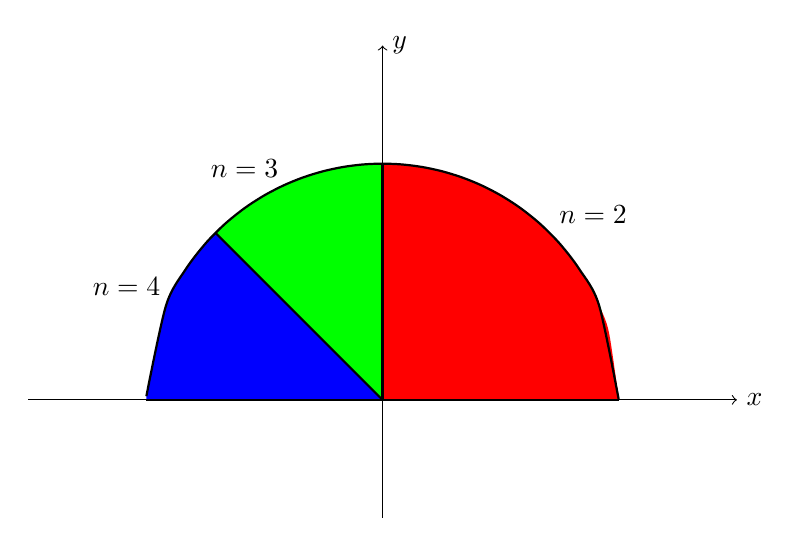
\begin{tikzpicture}[scale=3, smooth]
	\draw [->] (-1.5,0) -- (1.5,0) node[right]{$x$};
	\draw [->] (0,-0.5) -- (0,1.5) node[right]{$y$};
	
	\fill[fill=blue] (1,0) -- plot [domain=1:-1] (\x, {sqrt(1 - \x*\x)}) --
		(-1,0) -- (1,0);
	\fill[fill=green] (1,0) -- plot [domain=1:-0.707] (\x, {sqrt(1 - \x*\x)}) --
		(135:1) -- (0,0) -- (1,0);
	\fill[fill=red] (1,0) -- plot [domain=1:0] (\x, {sqrt(1 - \x*\x)}) --
		(0,0) -- (1,0);
	\draw [thick] (0,0) -- (1,0);
	\draw [thick] (0,0) -- ++ (90:1);
	\draw [thick] (0,0) -- ++ (135:1);
	\draw [thick] (0,0) -- ++ (180:1);
	\draw [thick] plot [domain=1:-1] (\x, {sqrt(1 - \x*\x});
	\node [above right] at (0.707, 0.707){$n = 2$};
	\node [above left] at  (-0.4, 0.9)   {$n = 3$};
	\node [above left] at  (-0.9, 0.4)   {$n = 4$};
\end{tikzpicture}
\end{center}


\textbf{4}
If $z$ follows the straight line $ay = x$, then the mapping $w = e^z$ is
\begin{align*}
	w &= e^{x + iy} \\
	&= e^{ay}e^{iy} \\
	&= e^{a\phi} e^{i\phi} \\
	&= \rho e^{i\phi}
\end{align*}
where $ \rho = a\phi$.


\textbf{5}
The rectangular region $a \le x \le b$, $c \le y \le d$ is made up of the horizontal line segments
\[
	x = t,	\quad	y = c_1
\]
where $t$ is a parameter running from $a$ to $b$ and $c_1$ is a constant in the range $[c, d]$. These horizontal lines have the images
\[
	\rho = e^t,	\quad	\phi = c_1
\]
Since $t$ starts at $a$ and ends at $b$, these images have a radius in the range $[e^a, e^b]$. Then, the entire image is the set of these lines, which range from $\phi = c$ to $\phi = d$. Thus, the entire image is
\[
	e^a \le \rho \le e^b,	\quad	c \le \phi \le d
\]


\textbf{6}
Looking at the $z$ plane, the initial set is the infinite strip
\[
	x \le 0, \quad	0 \le y \le \pi
\]
This maps to the image set
\[
	\lim_{a \to -\infty} e^{a} \le \rho \le e^0,	\quad 0 \le \phi \le \pi
\]
or
\[
	0 \le \rho \le 1,	\quad 0 \le \phi \le \pi
\]
This is the upper half of the unit disk, as shown in the figure.


\textbf{7}
In a similar manner to the previous problem, the image of the strip
\[
	x \ge 0, \quad	0 \le y \le \pi
\]
is the upper half-plane with a unit disk cut out:
\[
	\rho \ge 1,	\quad	0 \le \phi \le \pi
\]
A sketch of this region is:
\begin{center}
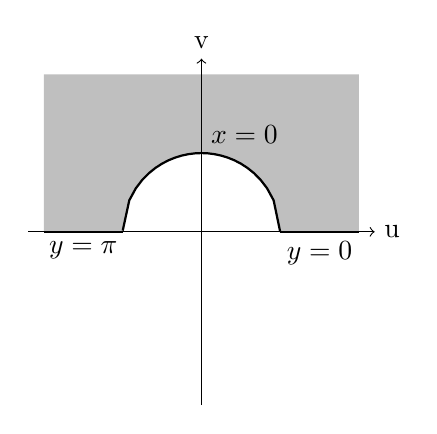
\begin{tikzpicture}	
	\fill [fill=gray!50] (2,0) -- (1,0) -- 
		plot [domain=1:-1] (\x, {sqrt(1 - \x*\x)}) --
		(-1,0) -- (-2,0) -- (-2,2) -- (2,2) -- (2,0);
		
	\draw [->] (-2.2,0) -- (2.2,0) node [right]{u};
	\draw [->] (0,-2.2) -- (0,2.2) node [above]{v};
	
	\draw [thick] (1,0) -- (2,0);
	\node [below] at (1.5,0) {$y = 0$};
	\draw [thick] (-1,0) -- (-2,0);
	\node [below] at (-1.5,0) {$y = \pi$};
	\draw [thick] plot [domain=1:-1] (\x, {sqrt(1 - \x*\x)});
	\node [above right] at (0,1) {$x = 0$};
\end{tikzpicture}
\end{center}


\textbf{8}
Some sample vectors in these two fields are:
\begin{center}
\begin{tikzpicture}
	\draw [->] (-5.5,0)  -- (-0.5,0) node [right]{$x$};
	\draw [->] (-3,-2.5) -- (-3,2.5) node [right]{$y$};
	
	\draw [thick, ->] (-3,0) ++ (1,0) -- ++(90 :0.5);
	\draw [thick, ->] (-3,0) ++ (2,0) -- ++(90 :1);
	\draw [thick, ->] (-3,0) ++ (0,1) -- ++(180:0.5);
	\draw [thick, ->] (-3,0) ++ (0,2) -- ++(180:1);
	\draw [thick, ->] (-3,0) ++ (-1,0) -- ++(270 :0.5);
	\draw [thick, ->] (-3,0) ++ (-2,0) -- ++(270 :1);
	\draw [thick, ->] (-3,0) ++ (0,-1) -- ++(0:0.5);
	\draw [thick, ->] (-3,0) ++ (0,-2) -- ++(0:1);
	
	
	\draw [->] (0.5,0)  -- (5.5,0) node [above right]{$x$};
	\draw [->] (3,-2.5) -- (3,2.5) node [right]{$y$};
	
	\draw [thick, ->] (3,0) ++ (1,0) -- ++(0:0.5);
	\draw [thick, ->] (3,0) ++ (2,0) -- ++(0:1);
	\draw [thick, ->] (3,0) ++ (0,1) -- ++(90:0.5);
	\draw [thick, ->] (3,0) ++ (0,2) -- ++(90:1);
	\draw [thick, ->] (3,0) ++ (-1,0) -- ++(180:0.5);
	\draw [thick, ->] (3,0) ++ (-2,0) -- ++(180:1);
	\draw [thick, ->] (3,0) ++ (0,-1) -- ++(270:0.5);
	\draw [thick, ->] (3,0) ++ (0,-2) -- ++(270:1);
\end{tikzpicture}
\end{center}


\clearpage
\section{Frame 18 -- Limits and Continuity}
\textbf{1(a)}
The left side of the limit is
\[
	|\Re(z) - \Re(z_0)| = |\Re(z - z_0)| < |z - z_0|
\]
so
\[
	|\Re(z) - \Re(z_0)| < \delta \text{ whenever } |z - z_0| < \delta
\]

\textbf{1(b)}
The left side of the limit is
\[
	|\bar{z} - \bar{z_0}| = |\bar{z - z_0}| = |z - z_0|
\]
so the limit holds.

\textbf{1(c)}
The limit expression is
\[
	|\frac{\bar{z}^2}{z}| < \epsilon \text{ whenever } |z| < \delta
\]
For $z \neq 0$, the left side expression is $|z|$, so the limit holds where $\epsilon = \delta$.

\textbf{2(a)}
The left side of the limit is
\[
	| (az + b) - (az_0 + b) | = |a(z - z_0)| = |a| |z - z_0|
\]
so the limit holds for $\delta = a \epsilon$.

\textbf{2(b)}
The left side is
\[
	| (z^2 + c) - (z_0^2 + c) | = |z^2 - z_0^2| = |z + z_0||z - z_0| \approx 2|z_0||z - z_0|
\]
for $\delta << |z_0|$. Thus, the limit holds for $\delta = 2z_0 \epsilon$. Note that if $z_0 = 0$, then this reduces to the limit of a constant value $c$, which is trivial.

\textbf{2(c)}
The right side is
\begin{align*}
	|z - (1 - i)| &= |[x - 1] + i[y + 1]| \\
	&= \sqrt{(x - 1)^2 + (y + 1)^2}
\end{align*}
The left side is
\begin{align*}
	| [x + i(2x + y)] - [1 + i] | &= | [x - 1] + i[2x + y - 1] | \\ 
	&= | [x - 1] + i[2(x - 1) + (y + 1)] | \\
\end{align*}
Not sure how to prove limits -- it appears as the right side goes to 0, the left side must too.

\textbf{3(a)}
If $z_0 \neq 0$, the limit must be
\[
	\lim_{z \to z_0} \frac{1}{z^n}
	= \frac{\lim_{z \to z_0} 1}{\lim_{z \to z_0} z^n}
	= \frac{1}{z_0^n}
\]

\textbf{3(b)}
\[
	\lim_{z \to i} \frac{iz^3 - 1}{z + i}
	= \frac{\lim{z \to i} iz^3 - 1}{\lim{z \to i} z + i} 
	= \frac{i(i^3) - 1}{(i) + i}
	= 0
\]

\textbf{3(c)}
\[
	\lim_{z \to z_0} \frac{P(z)}{Q(z)}
	= \frac{\lim_{z \to z_0} P(z)}{\lim_{z \to z_0} Q(z)}
	= \frac{P(z_0)}{Q(z_0)}
\]

\textbf{4}
The base case is
\[
	\lim_{z \to z_0} z = z_0
\]
which was shown earlier. 

If it is known that
\[
	\lim_{z \to z_0} z^k = z_0^k
\]
then the following limit is
\[
	\lim_{z \to z_0} z^{k+1} 
	= \left(\lim_{z \to z_0} z^k \right) \left(\lim_{z \to z_0} z \right)
	= (z_0^k)(z_0) 
	= z_0^{k+1}
\]
so, by induction, we are finished.

\textbf{5}
First, for any point $z = (x, 0)$, the function is
\[
	f(x, 0) = \left( \frac{x}{x} \right)^2 = (1)^2 = 1
\]
so the limit as $x \to 0$ is 1.

Then, for any point $z = (x, x)$, the function is
\[
	f(x, x) = \left( \frac{x + ix}{x - ix} \right)^2 = (i)^2 = -1
\]
so the limit as $x \to 0$ is $-1$. This conflicts with the previous result, so the limit does not exist.

\textbf{6(a)}
\textit{The statement to be proved is
\[
	\lim_{z \to z_0}[f(z) + F(z)] = w_0 + W_0
\]}

If $f$ and $F$ are split into their real and imaginary parts ($u$, $v$, $U$, and $V$), then we know that
\begin{align*}
	\lim_{z \to z_0} u(x, y) &= u_0 \\
	\lim_{z \to z_0} v(x, y) &= v_0 \\
	\lim_{z \to z_0} U(x, y) &= U_0 \\
	\lim_{z \to z_0} V(x, y) &= V_0
\end{align*}
Then, the sum $f(z) + F(z)$ has a real and imaginary part, which have the limits
\begin{align*}
	\lim_{z \to z_0} u(x, y) + U(x, y) &= u_0 + U_0 \\
	\lim_{z \to z_0} v(x, y) + V(x, y) &= v_0 + V_0 \\
\end{align*} 
so the result is
\[
	\lim_{z \to z_0} f(z) + F(z) = u_0 + v_0 + U_0 + V_0 = w_0 + W_0
\]

\textbf{6(b)}
The left side of the limit expression is
\begin{align*}
	|f(z) + F(z) - w_0 - W_0| &= |f(z) - w_0 + F(z) - W_0| \\
	&\le |f(z) - w_0| + |F(z) - W_0| \\
	&< \epsilon + \epsilon \\
	&= 2\epsilon
\end{align*}
so the statement is true, and the limit is $w_0 + W_0$.

\textbf{7}
The left hand side of the expression is
\[
	| |f(z)| - |w_0|| \le |f(z) - w_0|
\]
which is the standard limit expression. Since $\lim_{z \to z_0} f(z) = w_0$, this expression is true, and the limit is $|w_0|$.

\textbf{10(a)}
Making the replacement in the expression, this limit is
\begin{align*}
	\lim_{z \to \infty} \frac{4z^2}{(z - 1)^2} 
	&= \lim_{z \to 0} \frac{4(1/z)^2}{(1 - (1/z))^2} \\
	&= \lim_{z \to 0} \frac{4}{(z - 1)^2} \\
	&= \frac{4}{1} = 4
\end{align*}

\textbf{10(b)}
The reciprocal of this expression has the limit
\[
	\lim_{z \to 1} (z - 1)^3 = 0
\]
so the limit is infinity.

\textbf{10(c)}
Taking both reciprocals,
\begin{align*}
	\lim_{z \to \infty} \frac{z - 1}{z^2 + 1}
	&= \lim_{z \to 0} \frac{(1/z) - 1}{(1/z)^2 + 1} \\
	&= \lim_{z \to 0} \frac{z - z^2}{1 + z^2} \\
	&= \frac{0}{1} = 0
\end{align*}
so the limit is infinity.


\clearpage
\section{Frame 20 -- Differentiation}
\textbf{1}
These four derivatives are:
\begin{itemize}
	\item{(a)}
	\[
		\frac{d}{dz}(3z^2 - 2z + 4) = 6z - 2
	\]
	
	\item{(b)}
	\[
		\frac{d}{dz}(1 - 4z^2)^3 = 3(1 - 4z^2)^2(-8z) = -24z(1 - 4z^2)^2
	\]
	
	\item{(c)}
	\[
		\frac{d}{dz} \frac{z - 1}{2z + 1} = \frac{(1)(2z + 1) - (2)(z - 1)}{(2z + 1)^2} = \frac{-1}{(2z + 1)^2}
	\]
	
	\item{(d)}
	\begin{align*}
		\frac{d}{dz} \frac{(1 + z^2)^4}{z^2} 
		&= \frac{4(1 + z^2)^3(2z)(z^2) - 2z(1 + z^2)^4}{z^4} \\
		&= \frac{8z^3(1 + z^2)^3 - (2z + 2z^3)(1 + z^2)^3}{z^4} \\
		&= \frac{2z(3z^2 - 1)(1 + z^2)^3}{z^4}
	\end{align*}
\end{itemize}

\textbf{2}
First, each term of the polynomial $P_k(z)$ is
\[
	P_k(z) = a_k z^k
\]
All of these terms are differentiable everywhere, and the derivative is
\[
	P_k'(z) = k a_k z^{k-1}, \quad	k \neq 0
\]
where the derivative of $a_0$ is simply zero. Then, we proved that the derivative of a sum is the sum of two derivatives, so we can apply this repeatedly to find
\[
	P'(z) = a_1 + 2a_2 z + \dots + na_n z^{n-1}
\]

Notice that the function's value at zero is $P(0) = a_0$. The derivative's value at zero is similarly $P'(0) = a_1$. Applying the same process again, we find that
\begin{align*}
	P''(0) &= 2a_2 \\
\intertext{and}
	P^{(k)}(0) &= k! \cdot a_k
\end{align*}
Rearranging these terms, we can write
\begin{align*}
	a_0 &= P(0) \\
	a_1 &= \frac{P'(0)}{1!} \\
	a_2 &= \frac{P''(0)}{2!} \\
	&\dots \\
	a_n &= \frac{P^{(n)}(0)}{n!} 
\end{align*}

\textbf{3}
We can find the derivative of $f(z) = \frac{1}{z}$ by using the definition:
\[
	\frac{d}{dz} \frac{1}{z}
	= \lim_{\Delta z \to 0} \frac{\frac{1}{z + \Delta z} - \frac{1}{z}}{\Delta z}
	= \lim_{\Delta z \to 0} \frac{(z) - (z + \Delta z)}{z\Delta z (z + \Delta z)}
	= \lim_{\Delta z \to 0} \frac{-1}{z (z + \Delta z)}
	= \frac{-1}{z^2}
\]

\textbf{4}
Applying the definition of a derivative, we can see that
\begin{align*}
	\lim_{z \to z_0} \frac{f(z)}{g(z)} 
	&= \lim_{z \to z_0} \frac{f(z) - f(z_0)}{g(z) - g(z_0)} \\
	&= \lim_{z \to z_0} \frac{f(z) - f(z_0)}{z - z_0} \frac{z - z_0}{g(z) - g(z_0)} \\
	&= \frac{f'(z_0)}{g'(z_0)}
\end{align*}

\textbf{5}
Following the proof shown in the chapter, the derivative of a sum makes the term $\Delta w$ into
\[
	\Delta w = f(z + \Delta z) - f(z) + g(z + \Delta z) - g(z)
\]
Then, the derivative is
\begin{align*}
	\frac{d}{dz} [f(z) + g(z)] 
	&= \lim_{\Delta z \to 0} \frac{\Delta w}{\Delta z} \\
	&= \lim_{\Delta z \to 0} \frac{f(z + \Delta z) - f(z) + g(z + \Delta z) - g(z)}{\Delta z} \\
	&= \lim_{\Delta z \to 0} \frac{f(z + \Delta z) - f(z)}{\Delta z} + \lim_{\Delta z \to 0}\frac{g(z + \Delta z) - g(z)}{\Delta z} \\
	&= f'(z) + g'(z)
\end{align*}

\textbf{6}
\textit{Base case:} the derivative of $z^1$ is $1$.

\textit{$k+1$ case:} if the derivative of $z^k$ is $kz^{k-1}$, then the derivative of $z^{k+1}$ is
\[
	\frac{d}{dz} z^{k+1} 
	= \frac{d}{dz} (z^k)(z) 
	= (kz^{k-1})(z) + (z^k)
	= (k+1)z^k
\]
Therefore, by induction, we are done.

\textbf{7}
When $n$ is a negative integer, we can write $m = -n$ and rewrite the function as
\[
	f(z) = \frac{1}{z^m}
\]
Then, using the quotient rule, the derivative of this function is
\[
	f'(z)
	= \frac{(0)(z^m) - (1)(mz^{m-1})}{z^{2m}}
	= \frac{nz^{-n-1}}{z^{-2n}}
	= nz^{n-1}
\]
so the derivative formula is still valid.	

\textbf{8(a)}
The derivative of $f(z) = \Re z$ is
\[
	\frac{d}{dz} \Re z 
	= \lim_{\Delta z \to 0} \frac{\Re(z + \Delta z) - \Re z}{\Delta z}
	= \lim_{\Delta z \to 0} \frac{\Re (\Delta z)}{\Delta z}
\]
To show that this limit doesn't exist, consider a point $z_1 = (x,0)$. The limit from this direction then becomes
\[
	f'(x, 0) = \lim_{x \to 0} \frac{x}{x} 
	= 1
\]
Then, consider a different point $z_2 = (0, y)$. The limit this time is
\[
	f'(0, y) = \lim{y \to 0} \frac{0}{y} = 0
\]
Since the limit is different from these two directions, the derivative does not exist.

The proof for $\Im (z)$ is nearly identical.






\end{document}